\documentclass[tikz, border=0px]{standalone}
\usepackage{tikz}
\usetikzlibrary{shapes,arrows}

\tikzstyle{startstop} = [rectangle,rounded corners,minimum width=3cm,minimum height=1cm,align=center,draw=black, text width=2.5cm, fill=green!30]

\tikzstyle{therapy} = [trapezium, trapezium left angle =70, trapezium right angle=110, minimum width=2cm, minimum height = 1cm, centered,draw=black,align=center, text width=2cm, fill=orange!30]

\tikzstyle{decision} = [diamond, minimum width = 3cm, minimum height = 3cm, text centered, draw=black, text width = 2cm,align=center,fill=blue!30]

\tikzstyle{arrow} = [thick, ->, >=stealth]
\tikzstyle{doublearrow} = [<->, thick, >=stealth]

\begin{document}
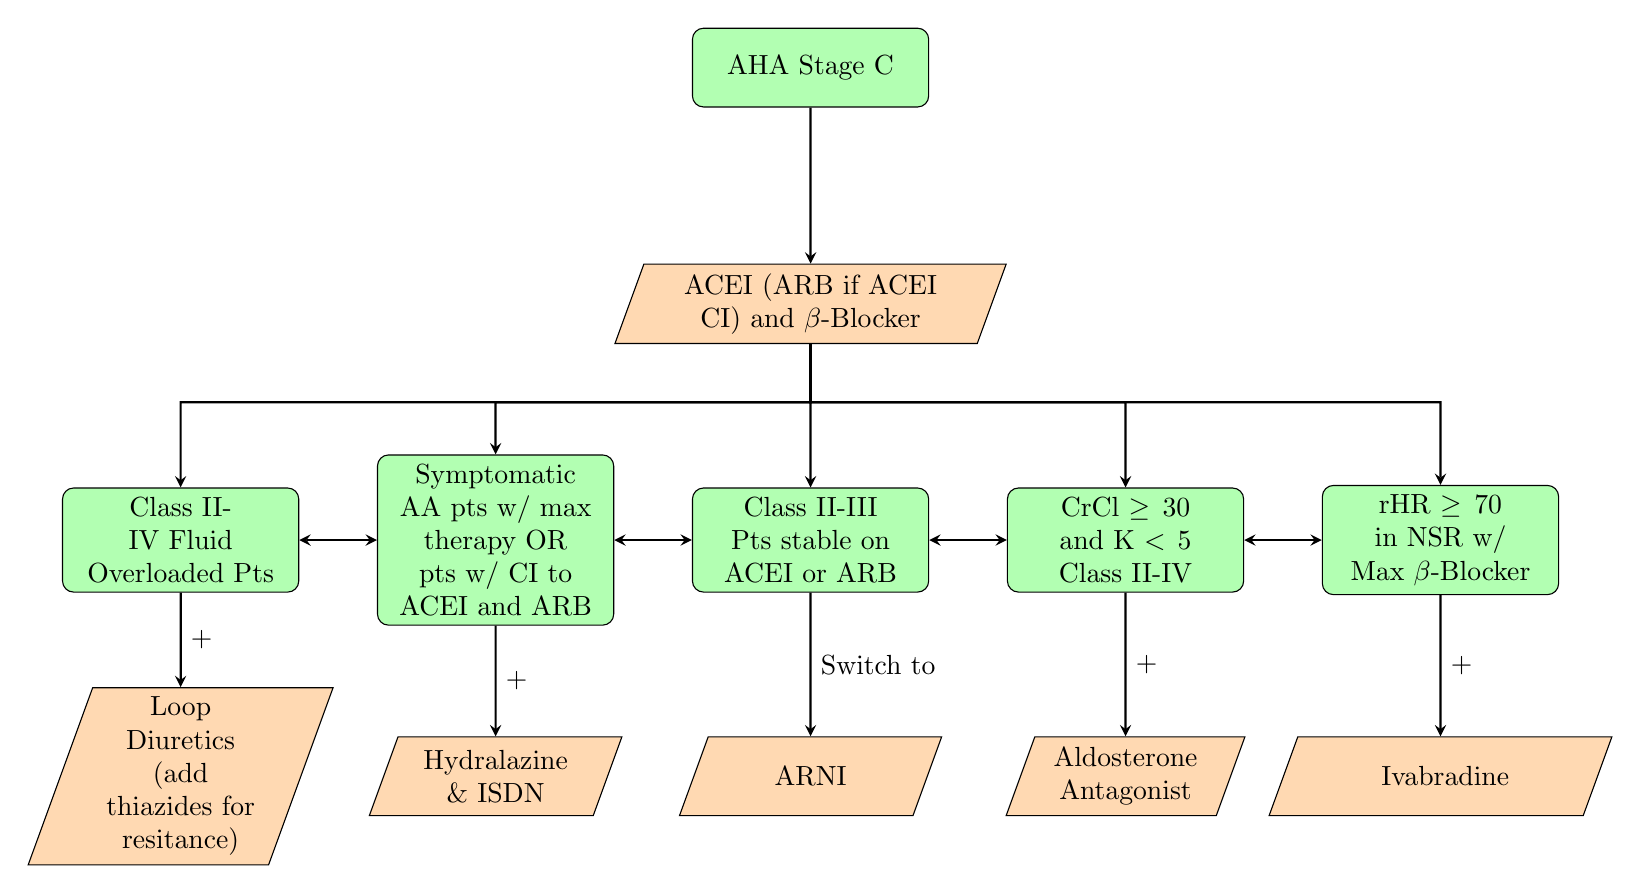
\begin{tikzpicture}[node distance=3cm]

\node (start) [startstop] {AHA Stage C};
\node (acei) [therapy, below of=start, text width=4cm] {ACEI (ARB if ACEI CI) and $\beta$-Blocker};

\node (diureticCriteria) [startstop, below of=acei, xshift=-8cm] {Class II-IV Fluid Overloaded Pts};
\node (diuretic) [therapy, below of=diureticCriteria] {Loop Diuretics (add thiazides for resitance)};

\node (bidilCriteria) [startstop, below of=acei, xshift=-4cm] {Symptomatic AA pts w/ max therapy OR pts w/ CI to ACEI and ARB};
\node (bidil) [therapy, below of=bidilCriteria] {Hydralazine \& ISDN};

\node (arniCriteria) [startstop, below of=acei, xshift=0cm] {Class II-III Pts stable on ACEI or ARB};
\node (arni) [therapy, below of=arniCriteria, text width=1cm] {ARNI};

\node (araCriteria) [startstop, below of=acei, xshift=4cm] {CrCl $\ge30$ and K $<5$ Class II-IV};
\node (ara) [therapy, below of=araCriteria] {Aldosterone Antagonist};

\node (ivabradineCriteria) [startstop, below of=acei, xshift=8cm] {rHR $\ge70$ in NSR w/ Max $\beta$-Blocker};
\node (ivabradine) [therapy, below of=ivabradineCriteria,text width = 1.5cm] {Ivabradine};

\draw [arrow] (start) -- (acei);
\draw [arrow] (acei) -- ++(0,-1.25cm) -| (diureticCriteria);
\draw [arrow] (acei) -- ++(0,-1.25cm) -| (bidilCriteria);
\draw [arrow] (acei) -- (arniCriteria);
\draw [arrow] (acei) -- ++(0,-1.25cm) -| (araCriteria);
\draw [arrow] (acei) -- ++(0,-1.25cm) -| (ivabradineCriteria);

\draw [arrow] (diureticCriteria) -- node[right] {+} (diuretic);
\draw [arrow] (bidilCriteria) -- node[right] {+} (bidil);
\draw [arrow] (arniCriteria) -- node[right] {Switch to} (arni);
\draw [arrow] (araCriteria) -- node[right] {+} (ara);
\draw [arrow] (ivabradineCriteria) -- node[right] {+} (ivabradine);

\draw [doublearrow] (diureticCriteria) -- (bidilCriteria);
\draw [doublearrow] (arniCriteria) -- (bidilCriteria);
\draw [doublearrow] (arniCriteria) -- (araCriteria);
\draw [doublearrow] (ivabradineCriteria) -- (araCriteria);




\end{tikzpicture}
\end{document}